%\title{LaTeX Portrait Poster Template}
%%%%%%%%%%%%%%%%%%%%%%%%%%%%%%%%%%%%%%%%%
% a0poster Portrait Poster
% LaTeX Template
% Version 1.0 (22/06/13)
%
% The a0poster class was created by:
% Gerlinde Kettl and Matthias Weiser (tex@kettl.de)
% 
% Adapter by Jens Buysse for Hogeschool Gent
% This template has been downloaded from:
% http://www.LaTeXTemplates.com
%
% License:
% CC BY-NC-SA 3.0 (http://creativecommons.org/licenses/by-nc-sa/3.0/)
%
%%%%%%%%%%%%%%%%%%%%%%%%%%%%%%%%%%%%%%%%%

%----------------------------------------------------------------------------------------
%	PACKAGES AND OTHER DOCUMENT CONFIGURATIONS
%----------------------------------------------------------------------------------------


\usepackage{multicol} % This is so we can have multiple columns of text side-by-side
\columnsep=100pt % This is the amount of white space between the columns in the poster
\columnseprule=3pt % This is the thickness of the black line between the columns in the poster

\usepackage[svgnames]{xcolor} % Specify colors by their 'svgnames', for a full list of all colors available see here: http://www.latextemplates.com/svgnames-colors

\usepackage{times} % Use the times font
%\usepackage{palatino} % Uncomment to use the Palatino font

\usepackage{graphicx} % Required for including images
\graphicspath{{figures/}} % Location of the graphics files
\usepackage{booktabs} % Top and bottom rules for table
\usepackage[font=small,labelfont=bf]{caption} % Required for specifying captions to tables and figures
\usepackage{amsfonts, amsmath, amsthm, amssymb} % For math fonts, symbols and environments
\usepackage{wrapfig} % Allows wrapping text around tables and figures
\usepackage[export]{adjustbox}

\begin{document}

%----------------------------------------------------------------------------------------
%	POSTER HEADER 
%----------------------------------------------------------------------------------------

% The header is divided into two boxes:
% The first is 75% wide and houses the title, subtitle, names, university/organization and contact information
% The second is 25% wide and houses a logo for your university/organization or a photo of you
% The widths of these boxes can be easily edited to accommodate your content as you see fit

\begin{minipage}[t]{0.75\linewidth}
\VeryHuge \color{HoGentAccent1} \textbf{Mag Webpack zich nog steeds de koning der Javascript build tools noemen?} \color{Black}\\ % Title
% \Huge\textit{Ondertitel (eventueel)}\\[2.4cm] % Subtitle
\huge \textbf{Vansteenkiste Maxim, Vanhaverbeke Cedric, Roobrouck Heidi}\\[0.5cm] % Author(s)
\huge Hogeschool Gent, Valentin Vaerwyckweg 1, 9000 Gent\\[0.4cm] % University/organization
\Large \texttt{maxim.vansteenkiste@student.hogent.be} \\
\end{minipage}
%
\begin{minipage}[t]{0.25\linewidth}

\includegraphics[width=13cm,right]{figures/HOGENT_Logo_Pos_rgb.png} 

\end{minipage}

\vspace{1cm} % A bit of extra whitespace between the header and poster content

%----------------------------------------------------------------------------------------

\begin{multicols}{2} % This is how many columns your poster will be broken into, a portrait poster is generally split into 2 columns

%----------------------------------------------------------------------------------------
%	ABSTRACT
%----------------------------------------------------------------------------------------

\color{HoGentAccent1} % Navy color for the abstract

\begin{abstract}
    Een Javascript build tool is een essentieel onderdeel bij het maken van moderne webapplicaties. Al jaren wordt Webpack gezien als de beste keuze hiervoor. Aangezien er genoeg andere opties zijn, vele met een nieuwe aanpak, is het wel eens tijd om die bewering te controleren. In een literatuurstudie wordt de geschiedenis en werking van een Javascript build tool geschetst. Daarna, aan de hand van een vergelijkende studie, worden drie populaire alternatieven tegenover Webpack geplaatst in rechtstreeks duel. Eerst wordt een nieuw project opgezet met de respectievelijke kandidaten. Daarna trachten we drie open-source projecten, elk met zijn eigen moeilijkheden, om te vormen van Webpack naar een tegenkandidaat. Doorheen dit gedocumenteerd proces, wordt er meer uitleg gegeven over de verschillende technologieën die aan bod komen. Tot slot wordt in de conclusie, rekening houdend met verschillende ob- en subjectieve factoren, de titel van deze proef beantwoord.
\end{abstract}
%----------------------------------------------------------------------------------------
%	INTRODUCTION
%----------------------------------------------------------------------------------------

\color{HoGentAccent1} 
\section*{Introductie}
\color{black}
\color{black}
De wijze waarop een webapplicatie gemaakt wordt, verandert continu. Het lijkt wel of er elke week een nieuw framework uitkomt met een iets andere aanpak dan al degene die hem voorgingen. Eén ding echter blijft al enkele jaren hetzelfde: de nood aan een build tool is er nog steeds, voor nu toch.

Dit onderzoek tracht de noodzaak, werking en toekomst van de Javascript build tool te schetsen. Dit aan de hand van een paar veel voorkomende implementaties ervan. Het uiteindelijke doel is om te bepalen of de huidige koning, Webpack, nog steeds het recht heeft om die titel op te eisen.

%----------------------------------------------------------------------------------------
%	GEOLOGY
%----------------------------------------------------------------------------------------

\color{Black} % DarkSlateGray color for the rest of the content
\color{HoGentAccent1} 
\section*{Experimenten}
\color{black}
Er bestaan veel verschillende Javascript build tools. Ze allemaal vergelijken zou onbegonnen werk zijn. Gelukkig werken velen op zo goed als dezelfde manier. 
Vier Javascript build tools werden gekozen, vergeleken en getest in deze proef. Eerst wordt een nieuw project opgezet. Daarna vormen we drie open-source projecten die met Webpack opgezet zijn, om naar een andere kandidaat. Zo proberen we een antwoord te achterhalen op de titel van dit werk.

\color{black}
\begin{center}\vspace{1cm}
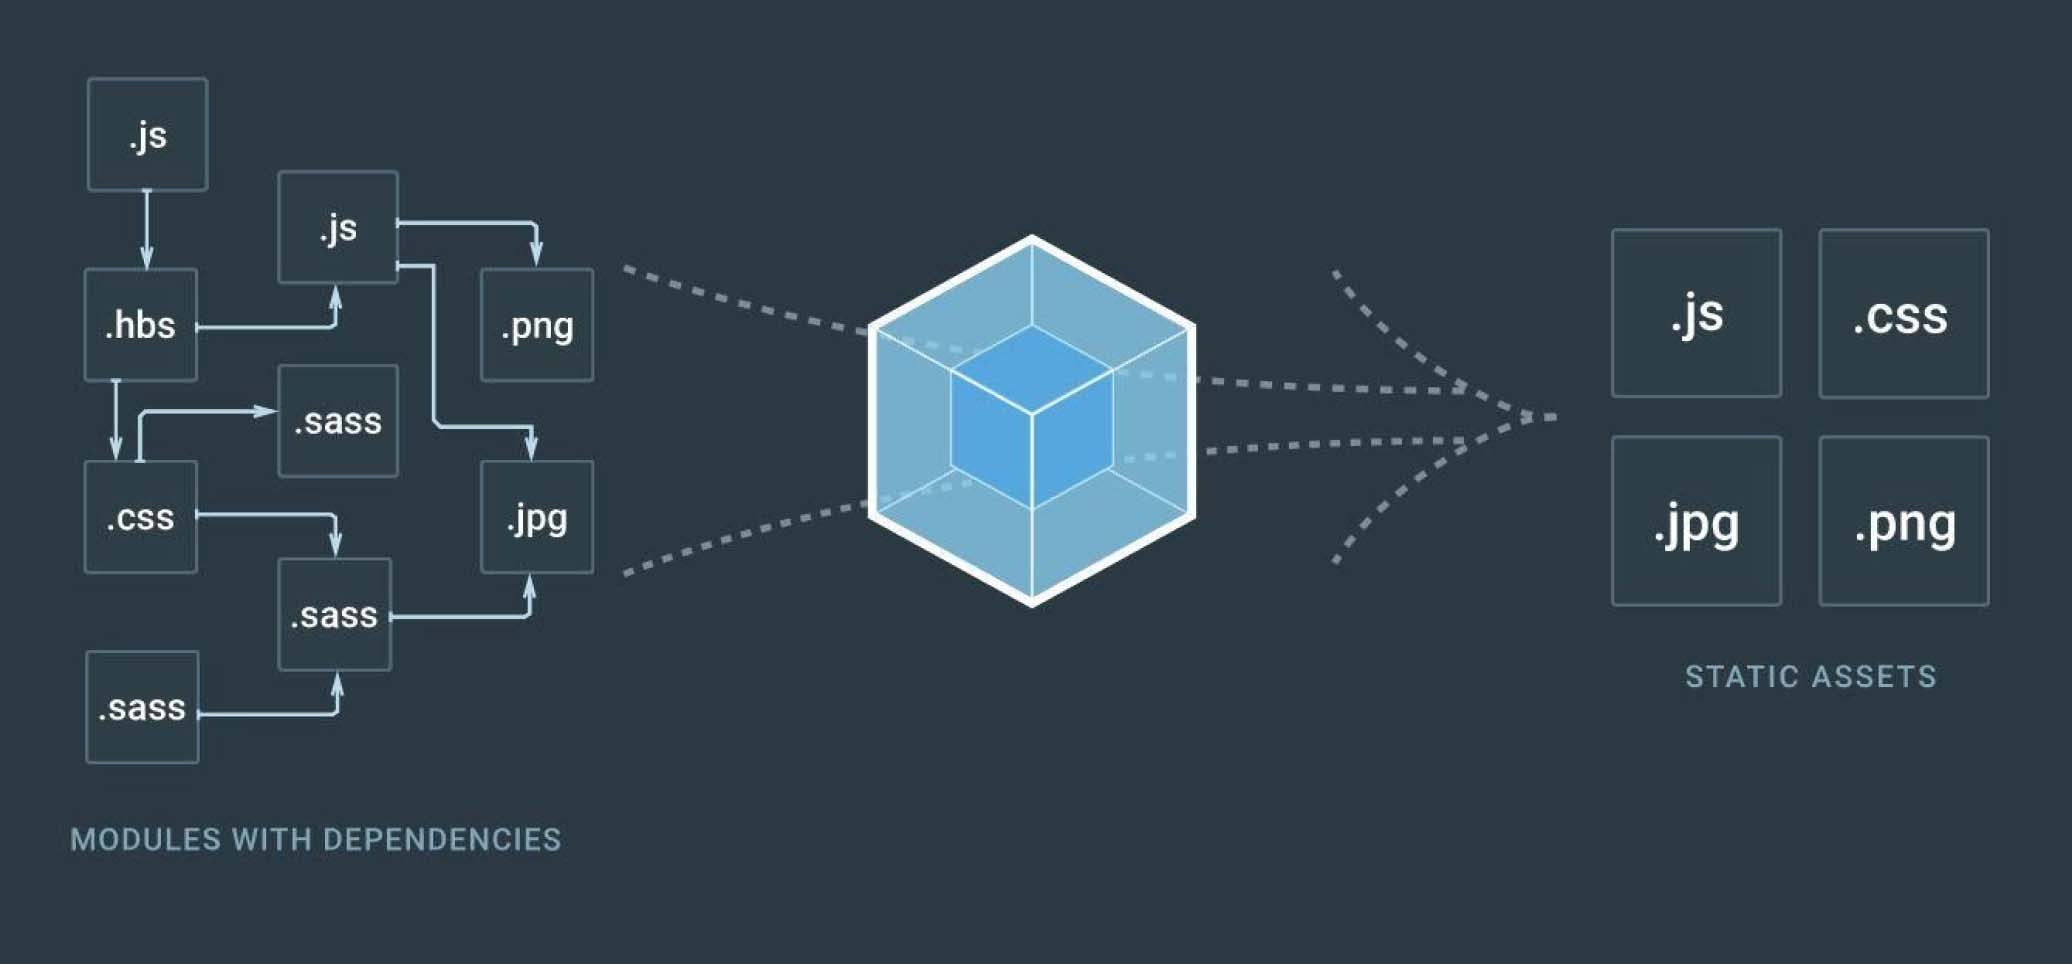
\includegraphics[width=1.0\linewidth]{./Webpack.jpg}
\captionof{figure}{Essentiële functie module bundlers (Webpack, g.d.-c)}
\end{center}\vspace{1cm}
%------------------------------------------------



\color{HoGentAccent1} 
\section*{Conclusies}
\color{black}
De hoofdvraag van deze proef, of Webpack nog steeds mag gezien worden als de koning der Javascript build tools, kan beantwoord worden met een duidelijke ‘nee’. Zelf binnen zijn eigen categorie van module bundlers, blijkt Parcel, in de meeste gevallen, een betere optie te zijn. Vite bewees dat de ongebundelde build tools de toekomst zijn. Module bundlers zijn hierdoor echter nog niet voorbijgestreefd. Zelfs wanneer browsers en Node.js ESModules volledig ondersteunen en alle open-source packages er volledig mee geschreven zijn, zullen de voordelen van module bundlers hun plaats in de Javascript wereld garanderen. Voor de nabije toekomst zullen module bundlers en ongebundelde build tools hand in hand moeten samenwerken om het beste van beide werelden samen te brengen. Vite lijkt dit het best te begrijpen. Het is dus wel duidelijk dat Vite de beste optie is voor zowel een nieuwe webapplicatie te ontwikkelen, als een bestaand een nieuwe, snellere en modernere motor te geven.
%----------------------------------------------------------------------------------------
%	FORTHCOMING RESEARCH
%----------------------------------------------------------------------------------------
\color{HoGentAccent1} 
\section*{Toekomstig onderzoek}
\color{black}

De wereld van webapplicatie ontwikkeling staat nooit stil. Het lijkt wel of er bijna iedere week een nieuw framework uitkomt. Hoewel het dus op dit moment nog zo is dat een build tool een module bundler nodig heeft, zal dat over enkele jaren misschien niet het geval zijn. De manier hoe developers hun webapplicaties bouwen of builden blijft onderhevig aan veranderingen en dus zal verder onderzoek nooit veraf zijn.

%----------------------------------------------------------------------------------------

\end{multicols}
\end{document}